%----------------------------------------------------------------------------------------
%	LATEX LABBOOK TEMPLATE
%	Versie 1.0 (12 september 2013)
%	Opmerkingen of feedback naar Robert van Wijk
%					(robertvanwijk@uva.nl)
%----------------------------------------------------------------------------------------

%----------------------------------------------------------------------------------------
%	PACKAGES EN DOCUMENT CONFIGURATIE
%----------------------------------------------------------------------------------------

\documentclass[a4paper,12pt]{article}
\usepackage{graphicx}
\usepackage[english]{babel}
\usepackage{fancyhdr}
\usepackage{lastpage}
\usepackage{xifthen}

\usepackage{DejaVuSansMono}
\usepackage{microtype}
\usepackage{mathtools}
\usepackage{textcomp}

%----------------------------------------------------------------------------------------
%	HEADER & FOOTER
%----------------------------------------------------------------------------------------

\pagestyle{fancy}
  \lhead{
\includegraphics[width=7cm]{logoUvA}}
  \rhead{\footnotesize \textsc {Technisch rapport\\ \opdracht}}
  \lfoot
    {
	\ifthenelse{\isundefined{\studentB}}{}{\\ \studentB}
	\ifthenelse{\isundefined{\studentC}}{}{\\ \studentC}
	\ifthenelse{\isundefined{\studentD}}{}{\\ \studentD}
	\ifthenelse{\isundefined{\studentE}}{}{\\ \studentE}
	Groep 5
    }
  \cfoot{}
  \rfoot{\small \textsc {Pagina \thepage\ van \pageref{LastPage}}}
  \renewcommand{\footrulewidth}{0.5pt}

\fancypagestyle{firststyle}
 {
  \fancyhf{}
   \renewcommand{\headrulewidth}{0pt}
   \chead{
\includegraphics[width=7cm]{logoUvA}}
   \rfoot{\small \textsc {Pagina \thepage\ van \pageref{LastPage}}}
 }

\setlength{\topmargin}{-0.3in}
\setlength{\textheight}{630pt}
\setlength{\headsep}{40pt}

%----------------------------------------------------------------------------------------
%	DOCUMENT INFORMATIE
%----------------------------------------------------------------------------------------

\newcommand{\titel}{A Poorman's MIPS Architecture}
\newcommand{\opdracht}{}
\newcommand{\docent}{Prof. dr. Jan van Eijck}
\newcommand{\cursus}{Functional Specification of Algorithms}
\newcommand{\datum}{\today}
\newcommand{\studentA}{David Veenstra}
\newcommand{\uvanetidA}{10094423}
%\newcommand{\studentB}{}
%\newcommand{\uvanetidB}{}
%\newcommand{\studentC}{Naam student 3}
%\newcommand{\uvanetidC}{UvAnetID student 3}
%\newcommand{\studentD}{Naam student 4}
%\newcommand{\uvanetidD}{UvAnetID student 4}
%\newcommand{\studentE}{Naam student 5}
%\newcommand{\uvanetidE}{UvAnetID student 5}
%\newcommand{\binom1}[1][2]{\left(\! \begin{array}{c} #1 \\ #2 \end{array}
%\!\right)}
\newcommand{\barg}[1]{\textlangle{}#1\textrangle{}}
\newcommand{\reg}[1]{\$#1}
\newcommand{\norm}[1]{|| #1 ||}

%----------------------------------------------------------------------------------------
%	AUTOMATISCHE TITEL
%----------------------------------------------------------------------------------------
\begin{document}
\thispagestyle{firststyle}
\begin{center}
	\textsc{\Large \opdracht}\\[0.2cm]
		\rule{\linewidth}{0.5pt} \\[0.4cm]
			{ \huge \bfseries \titel}
		\rule{\linewidth}{0.5pt} \\[0.2cm]
	{\large \datum  \\[0.4cm]}

	\begin{minipage}{0.4\textwidth}
		\begin{flushleft}
			\emph{Student:}\\
			{
        \ifthenelse{\isundefined{\studentA}}{}{\studentA \\ {\small \uvanetidA \\[0.2cm]}}
        \ifthenelse{\isundefined{\studentB}}{}{\studentB \\ {\small \uvanetidB \\[0.2cm]}}
				\ifthenelse{\isundefined{\studentC}}{}{\studentC \\ {\small \uvanetidC \\[0.2cm]}}
				\ifthenelse{\isundefined{\studentD}}{}{\studentD \\ {\small \uvanetidD \\[0.2cm]}}
				\ifthenelse{\isundefined{\studentE}}{}{\studentE \\ {\small \uvanetidE \\[0.2cm]}}
				}
		\end{flushleft}
	\end{minipage}
~
	\begin{minipage}{0.4\textwidth}
		\begin{flushright}
			\emph{Docent:} \\
			\docent \\[0.2cm]
			\emph{Course:} \\
			\cursus \\[0.2cm]
		\end{flushright}
	\end{minipage}\\[1 cm]
\end{center}

%----------------------------------------------------------------------------------------
%	INHOUDSOPGAVE EN ABSTRACT
%----------------------------------------------------------------------------------------

%\tableofcontents
%\begin{abstract}
%\end{abstract}

%----------------------------------------------------------------------------------------
%	INHOUD
%----------------------------------------------------------------------------------------

\section{Introduction}
% connection between arrows and frp
% why yampa
% implementation should be as close as possible as the original
% benefits of these abstractions 1. guidelines for dev 2. consistency of
% notation 3. freebies

Haskell has a treasure chest full of interesting abstraction, often borrowed or
inspired by category theory. The monoid, the functor and the monad abstractions are a few
examples. Especially the last one, the monad, has been of great importance, as
it allowed an otherwise pure language to deal with IO operations in elegant
manner. 

Besides the more common abstractions mentioned above, Haskell also have a number
of more exotic abstractions, such as the lens, comonad, bifunctor, profunctor
and arrow. This paper will take a look at the arrow abstraction.

Arrows where originally designed to solve a problem with parser combinators
using monads, such as the \emph{parsec} library. The problem is simple. 
A parser cannot partially discard the input to save memory while parsing,
because the parser might fail, where upon an alternative parser might need to be
applied on the entire input.

Arrows can be seen as a circuit, and the combinators can be used
to build larger circuit existing out of smaller circuits. 

One of Haskell advantages is that often an implementation can be given that is
idiomatic in the specific domain of the problem. Again the parser combinators
are a great example, the resulting implementation often has a strong resemblance
to the grammar of what has to be parsed. Given the similarity between circuits
and arrows it is to be expected that it should be natural to simulate a computer
architecture with the use of arrows.

Another advantages of Haskell, is that composition has a central position. 

This paper will evaluate arrows as an abstraction of computation, by implementing a simple
computer architecture. In particular, arrows will be evaluated on the ease of
use, and how idomatic the implementation is in the domain of the problem.

This paper is structured as follows. Firstly, an introduction to arrows is
given and a few details of the yampa library are highlighted. Subsequently, the
PIPS architecture is outlined. Thirdly, the details of the implementation are
presented. Afterwards some crude benchmark are given for the simulation. And
finally the evaluation of arrows as an abstraction is given.

% startup the story
% purpose of article
% evaluation criteria
% outset of article
\section{Arrows}
\begin{align*}
  m &= \frac{|(\vec{x_0} - \vec{x_1})\vec{w}|}{\norm{\vec{w}}} \\
  &= \frac{|(-1 - b) - (1 -b)|}{\norm{\vec{w}}} \\
  &= \frac{|-2|}{\norm{ \vec{w} }} \\
  &= \frac{2}{ \norm{\vec{w}} } 
\end{align*}

\subsection{Yampa}
% Explain arrow based, for frp and simulation, arrow some protection against
% time leaks.
% reactimate
% io action > funcitonal part > io action
% part about state
% part about switching, but is not relevant

\section{Pips}
The poorman's Mips architecture, or Pips in short, is a simple, single cycle
architecture, with no fancy features like pipelining or caching. Similar to the
Mips architecture, all instructions have the same width. In this case, one
instruction can be represented by a 32-bit number. Furthermore, Pips has a
registry and memory where it can store 32-bit numbers, and it has logic to
perform integer arithmetic and conditional jumps.

The execution of one instruction is completed in one cycle. This process can be
split into three different stages. In the first stage the instruction is fetched
from the instruction memory and it is decoded. Based on this information, the
control unit sends signals to the different components to configure their operations. In
the second stage, the needed values are loaded from the registry if needed and the
Arithmetic Logic Unit (ALU) can be used to perform integer arithmetic. In the
final stage, data can be written back to the registery or data can be stored
into or loaded from memory. And it is calculated which instruction has to be
executed next.

The instruction set of Pip is subset of the official Mips instruction set.
See Table \ref{instruction-table} for the different instruction and their
syntax.

Figure \ref{pips-schematic} show a schematic of the architecture.
Some simplification were made. First, the instruction that is retrieved from
the instruction memory is a 32-bit number; the field that are split from the
instruction vary in the number of bits. Because some components expect input
with a certain number of bits, extra hardware is needed for compatibility.
However, in the simulation this hardware is left out, as it would be
represented by 32-bits number regardless. Second, the memory in MIPS is
byte-addressed, the PIPS architecture is word-addressed. And finally, the
schematic doesn't show the control unit and the control lines to prevent clutter.

The instruction retrieval and decoding can be seen on the left.
The 32-bit number that is retrieved is split in different
ways and in different fields, and is send to the control unit, the register,
the PC mutex and ALU mutex.

The second stage can be seen in the middle of the schematic. The ALU performs
binaire operation. The first argument originates from the register. To determine
the second argument, the ALU mutex is used. This can, for example, be
the memory address, in a LW or SW instruction. In addition to the result of the
binary operator, the ALU also has a second output, which is 1 if the result is
0, and return 0 otherwise. This is useful for the branch instructions.

The third stage can be seen on the right and upper part of the schematic.
The control unit determines if data has to written to the register, or to memory.
The writeback mutex is used to determine what data has to be written back to the
register. The PC mutex determines what the next program counter is, which
determines what instruction is fetched in the next cycle.

\begin{table}[h]
    \begin{tabular}{ l l l }

    Syntax & Example & Semantics\\
    \hline
   ADD \barg{reg}, \barg{reg}, \barg{reg} & ADD \$res, \$1, \$2 & $\$res = \$1 + \$2$
\\ SUB \barg{reg}, \barg{reg}, \barg{reg} & SUB \$res, \$1, \$2 & $\$res = \$1 - \$2$
\\ AND \barg{reg}, \barg{reg}, \barg{reg} & AND \$res, \$1, \$2 & $\$res = \$1 \mathrel{\&} \$2$
\\ OR \barg{reg},  \barg{reg}, \barg{reg} & OR \$res, \$1, \$2  & $\$res = \$1 \mathrel{|} \$2$
\\ XOR \barg{reg}, \barg{reg}, \barg{reg} & XOR \$res, \$1, \$2 & $\$res = \$1 \mathbin{\oplus} \$2$
\\ SLT \barg{reg}, \barg{reg}, \barg{reg} & SLT \reg{res}, \reg{1}, \reg{2}
& $\reg{res} = \begin{cases}1 & \reg{1} < \reg{2},\\ 0 & \text{otherwise} \end{cases}$
%
\\ SLL \barg{reg}, \barg{reg}, \barg{imm} & SLL \$res, \$1, 16 & $\$res = \$1 \ll 16 $
\\ SRL \barg{reg}, \barg{reg}, \barg{imm} & SRL \$res, \$1, 16 & $\$res = \$1 \gg 16 $
\\ ADDI \barg{reg}, \barg{imm} & ADDI \$res, \$1, 10 & $\$res = \$1 - 10 $
\\ LUI \barg{reg}, \barg{reg}, \barg{imm} & LUI \$res, 10     & $\$res = \$1 \mathrel{|} (10 \ll 16) $
%
\\ LW \barg{reg}, \barg{label}, \barg{reg} & LW \$el, array, \$index & $\$el = Mem[\reg{array} + \reg{index}]$
\\ SW \barg{reg}, \barg{label}, \barg{reg} & SW \$index, array, \$el & $Mem[\reg{array }+ \reg{index}] = \$el$
%
\\ BEQ \barg{reg}, \barg{reg}, \barg{label} & BEQ \$1, \reg{2}, Loop & jump to Loop if $\reg{1} = \reg{2}$
\\ BNE \barg{reg}, \barg{reg}, \barg{label} & BNE \$1, \reg{2}, Loop & jump to Loop if $\reg{1} \neq \reg{2}$
%
\\ J \barg{label}  & J Exit     & jump to label Exit
\\ JR \barg{label} & JR \reg{3} & jump to instruction \reg{3}
    \end{tabular}
    \centering
    \caption{Pips Instruction Set}
    \label{instruction-table}
\end{table}

% explain simplified Architecture, with no pipeline and cache or branch predictors
% explain that it is has integer arithmetic, which should still be turing complete
% explain the instructions that are available
% give diagrams of pips
\begin{figure}[h!]
    \centering
    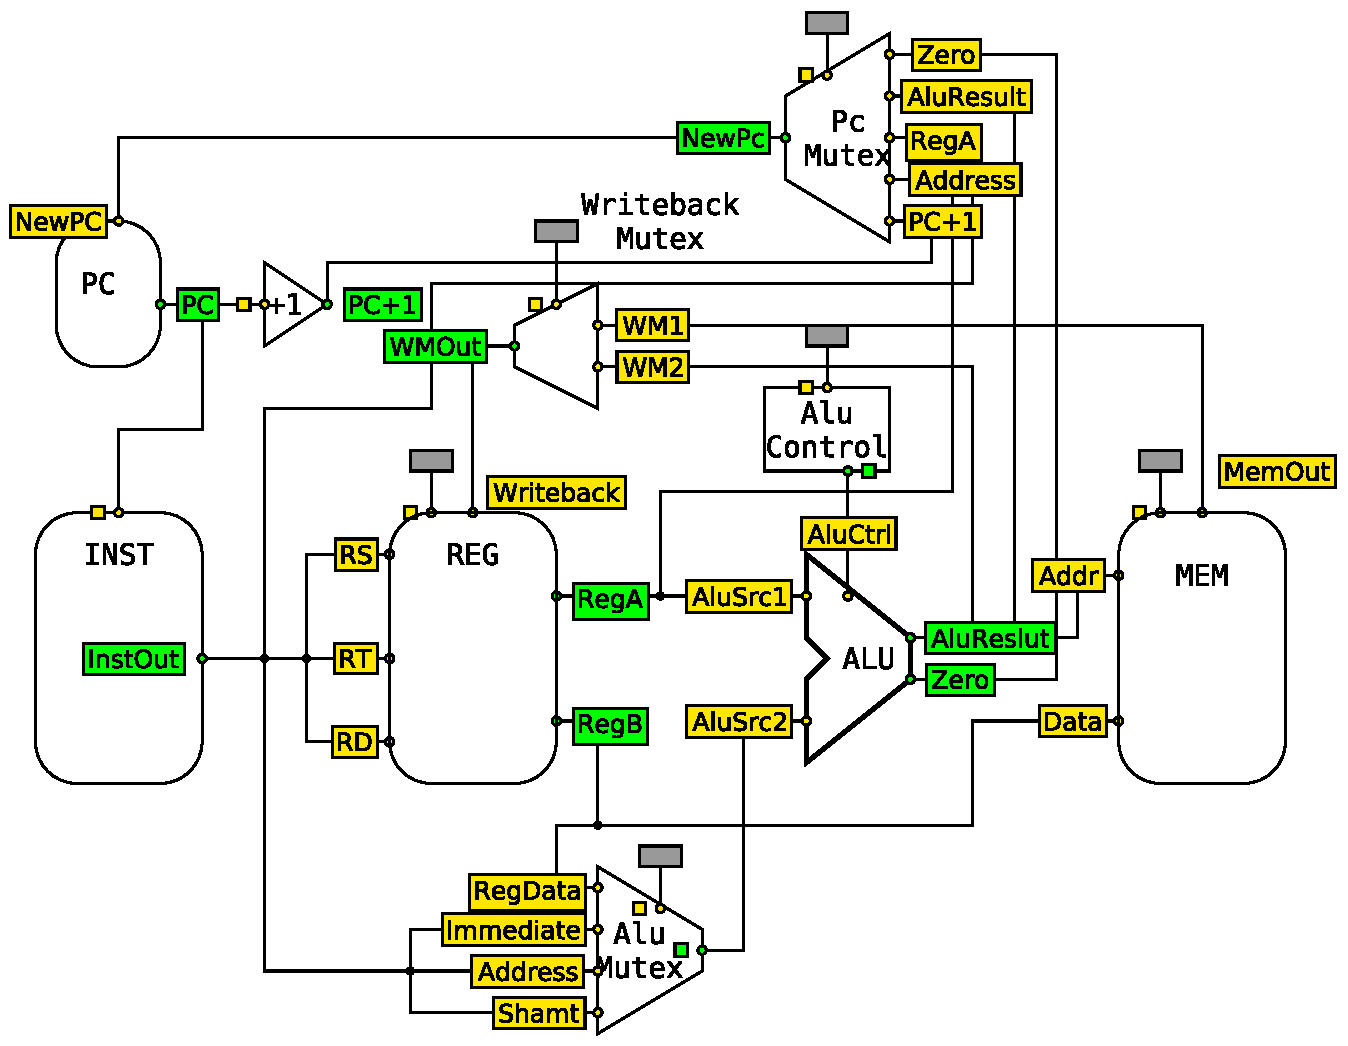
\includegraphics[width=\textwidth]{pips.pdf}
    \caption{Schematic of the Pips instruction. A green labels indicate an
      output port. A yellow label indicate an input port. The components that
      are connect to the gray boxes, are connected to the Control Unit.}
    \label{pips-schematic}
\end{figure}

\section{Implementation}
% explain how things have to be syncronised
% show the clock
% show the working of the register, and that is it similar to memory
% show the alu mutex
% show the alu
% show a simplified architecture, with some simplification

\subsection{Benchmark}
% show some benchmark on some programs 1. fib 2. multiplication algorithm 3.
% matrix multiplication or some other memory intensive program
% mention that it is a very crude benchmark
\begin{table}[h]
    \begin{tabular}{ l c c }
    
    Experiment& \multicolumn{2}{c}{Dataset} \\
    & Origineel & Gereduceerd \\
    \hline
    random split*    & 0.755454545455 & 0.812785388128 \\ 
    cross-validation & 0.735454545455 & 0.748858447489 
    
    \end{tabular}
    \centering
    \caption{De precisie van de SVM classifier bij de verschillende experimenten. *Gezien dit experiment niet deterministisch is, is het gemiddelde van tien pogingen gebruikt.}
    \label{accuracy}
\end{table}

\section{Evaluation}
% takes a while to get started just like monads -> progress goes to a crawl.
% the loops require some implicit properties throughout the whole program,
% that might result in circular loops
% Program looks very similar to schema. So familiar that it kinda has same
% problems as manualy wiring a it.
% biggest hurdle was syncronisation, rest was fairly straith forward.
% although the semantics of a SF a b is fairly similar to that of a function
% all the combinators present in arrows and yampa powerful enough to implement
% simulation.
% reason can be limited to component, each component can be tested fairly easily
% in hindsight this properly overkill to use yampa, as it is built for continues
% signal, while this was a discrete simulation.

\section{Discussion}

%----------------------------------------------------------------------------------------
%	REFERENTIES
%----------------------------------------------------------------------------------------

%\bibliographystyle{acm}
%\bibliography{biblliografie}

%----------------------------------------------------------------------------------------
%	BIJLAGEN
%----------------------------------------------------------------------------------------

%\section{Bijlage A}
%\section{Bijlage B}
%\section{Bijlage C}

\end{document}